\documentclass{article}

\usepackage{url}
\usepackage[hmargin=1.5in]{geometry}
\usepackage{enumitem}
\usepackage{amsmath}
\usepackage{amssymb}
\usepackage{amsthm}
\usepackage{eqnarray}
\usepackage{graphicx}
\usepackage[svgnames]{xcolor} %% for revisions
\usepackage{xparse} %% for squiggly underlines
\usepackage{tikz-cd} %% for term norm scratch work
\usepackage{tikz}

% TikZ libraries
\usetikzlibrary{bbox}
\usetikzlibrary{fadings}

% hat tip TeX.SE user marsupilam - https://tex.stackexchange.com/a/351570/6934
%%\tikzfading[
%%  name=radial,
%%  inner color=transparent!0,
%%  outer color=transparent!100
%%]
% hat tip TeX.SE user Andrew Stacey
%   https://tex.stackexchange.com/a/82503/6934
%   https://tex.stackexchange.com/questions/82425/tikz-radial-shading-of-a-ring#comment176908_82503
\pgfdeclareradialshading{infinifade}{\pgfpointorigin}{%
  color(0bp)=(transparent!0);
  color(20bp)=(transparent!0);
  color(22bp)=(transparent!10);
  color(24bp)=(transparent!90);
  color(25bp)=(transparent!100)
}
\pgfdeclarefading{infinity}{\pgfuseshading{infinifade}}%

%%\theoremstyle{definition}
\newtheorem{defn}{Definition}
\theoremstyle{plain}
\newtheorem{prop}{Proposition}
\newtheorem{thm}{Theorem}
\newtheorem{rmk}{Remark}

% format lists
\setlist[itemize]{leftmargin=15mm}
\makeatletter
% hat tip TeX.SE user31729
%   https://tex.stackexchange.com/a/328393/6934
\newcommand{\cond}[1]{\item[(\textsc{#1})]\protected@edef\@currentlabel{\textsc{#1}}}
\makeatother

% convenience aliases
\newcommand{\maps}{\colon}

% group action
\newcommand{\acts}{\mathbin{\raisebox{\depth}{\rotatebox{-90}{$\circlearrowright$}}}}

% symbology
\newcommand{\Z}{\mathbb{Z}}
\newcommand{\R}{\mathbb{R}}
\newcommand{\C}{\mathbb{C}}
\let\Re\relax
\DeclareMathOperator{\Re}{Re}
\newcommand{\laplace}{\mathcal{L}}
\newcommand{\series}[1]{\tilde{#1}}
\newcommand{\fracderiv}[3]{\partial^{#1}_{#2, #3}}

% function spaces
\newcommand{\cont}{\mathcal{C}}
\newcommand{\holo}{\mathcal{H}}
\newcommand{\singexp}[2]{\mathcal{H}L^\infty_{#1, #2}}
\newcommand{\holoL}[1]{\mathcal{H}L^{#1}} %% may no longer be needed
\newcommand{\expHoloL}[2]{\mathcal{H}L^{#1}_{#2}} %% may no longer be needed

% operator under consideration
\newcommand{\volterra}{\mathcal{V}}
\newcommand{\hardpart}{\mathcal{V}_\text{basic}}
\newcommand{\softpart}{\mathcal{V}_\text{extra}}
\newcommand{\hardker}{k_\text{basic}}
\newcommand{\softker}{k_\text{extra}}

% domain
\newcommand{\domain}{\Omega}
\newcommand{\near}{\Omega_\text{near}}
\newcommand{\far}{\Omega_\text{far}}

% drafting environments
\newenvironment{verify}{\color{ForestGreen}}{\color{black}}

\title{Regular singular Volterra equations on complex domains}
\author{Aaron Fenyes and Veronica Fantini}
\date{}

\begin{document}
\maketitle
\section{Introduction}
\subsection{Motivation}\label{motivation}
In its most basic form, the Laplace transform $\laplace$ turns $L^1$ functions of a real ``position'' variable $\zeta$ into holomorphic functions of a complex ``frequency'' variable $z$. Through identities like
\begin{align*}
\frac{\partial}{\partial z} \laplace \varphi & = \laplace(z\varphi) \\
\laplace k\;\laplace \varphi & = \laplace(k * \varphi) \\
z^{-\lambda} \laplace \varphi & = \laplace\,\fracderiv{-\lambda}{}{} \varphi,
\end{align*}
where $\fracderiv{-\lambda}{}{}$ is the Riemann-Liouville fractional integral of order $\lambda \in (0, \infty)$, the Laplace transform pulls differential operators on the frequency domain back to Volterra integral operators on the position domain. The favorable regularity properties and comprehensive theory of Volterra equations can thus be brought to bear on differential equations.

If we complexify the position variable $\zeta$, the functions on the position domain whose Laplace transforms satisfy a given differential equation will often extend holomorphically. \textbf{[...]}
\subsection{Setting}
\subsubsection{The domain}\label{setting:domain}
Throughout this paper, as described in Section~\ref{motivation}, the ``position'' variable $\zeta$ will be the standard coordinate on $\C$. Take a simply connected open set $\domain \subset \C$ that touches but doesn't contain $\zeta = 0$. For some of our results, we'll need an extra condition on $\domain$:
\begin{itemize}
\cond{star}\label{cond:star} The set $\domain$ is star-shaped around $\zeta = 0$. In other words, for any $a \in \domain$, a straight path from $\zeta = 0$ to $a$ stays in $\domain$. Since $\domain$ doesn't contain $\zeta = 0$, we'll always leave that starting point out of the path.
\end{itemize}
For the applications we have in mind, $\domain$ might look something like the set pictured below, which satisfies Condition~\eqref{cond:star}.
\begin{center}
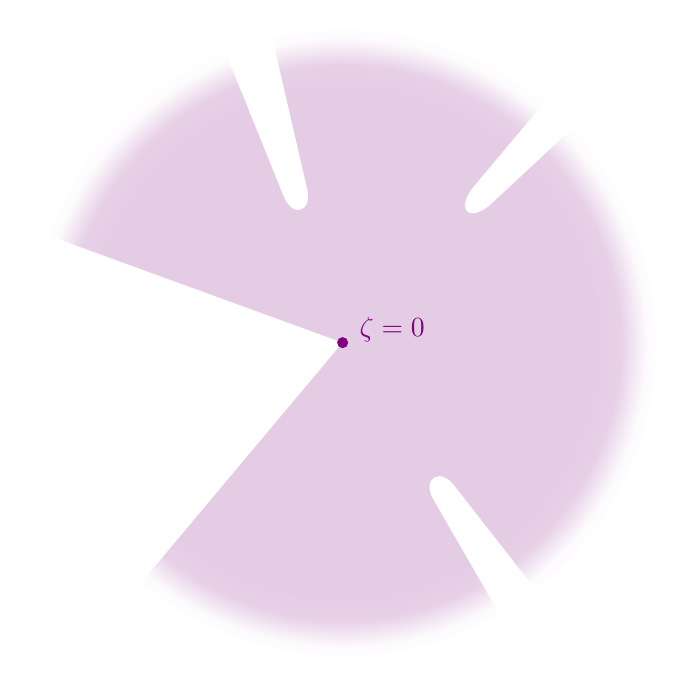
\begin{tikzpicture}
\newcommand{\spill}{4}
\fill[violet!20, bezier bounding box, path fading=infinity]
  (-\spill, -\spill) (\spill, \spill)
  (0, 0) -- (160:\spill)
  arc (160:112:\spill) -- (112:2) .. controls (112:1.7) and (103:1.7) .. (103:2) -- (103:\spill)
  arc (103:50:\spill) -- (50:2.6) .. controls (50:2.2) and (43:2.2) .. (43:2.6) -- (43:\spill)
  arc (43:-52:\spill) -- (-52:2.3) .. controls (-52:2) and (-60:2) .. (-60:2.3) -- (-60:\spill)
  arc (-60:-130:\spill) -- (0, 0);
\fill[violet] circle (0.7mm) node[anchor=195, outer sep=1mm] {$\zeta = 0$};
\end{tikzpicture}
\end{center}
\subsubsection{The prototype operator}\label{setting:basic}
The prototypical example of the kind of operator we'll be working with is a holomorphic Volterra operator $\hardpart$ with a separable kernel and a regular singularity at $\zeta = 0$.

Being a holomorphic Volterra operator means that $\hardpart$ sends each holomorphic function $\varphi$ on $\domain$ to a new holomorphic function
\[ [\hardpart\,\varphi](a) = \int_{\zeta = 0}^a \hardker(a, \cdot)\,\varphi\;d\zeta. \]
Being separable means that the kernel $\hardker(a, a')$ factors into a function of $a$ times a function of $a'$. We'll suppose this product can be written as a ratio
\[ \hardker(a, a') = \frac{q(a')}{p(a)}, \]
where $p$ and $q$ are holomorphic functions on $\domain$. Having a regular singularity at $\zeta = 0$ means that for some constant $\tau$---the {\em residue} of the singularity---the difference
\[ -\frac{\tau}{\zeta(a)} - \hardker(a, a') \]
is bounded on a neighborhood of $\big(\zeta(a), \zeta(a')\big) = (0, 0)$ in $\Omega^2$. We'll assume that $\tau$ is real and positive.

Our definition of a regular singularity implies that as $|\zeta|$ goes to zero, $|p|$ also goes to zero, while $|q|$ settles into a compact interval that doesn't include zero.
\begin{verify}
[\textit{Proof.} Fix any $a'$ in the neighborhood where the difference above is bounded. By confining $a$ to small enough neighborhoods of $\zeta = 0$, we can make $|\tau/\zeta(a)|$ arbitrarily large, forcing $|q(a')/p(a)|$ to become arbitrarily large to satisfy the definition. Since $a'$ is fixed, the only way for this ratio to get arbitrarily large is for $|p(a)|$ to get arbitrarily small.]
\end{verify}
For some of our results, we'll also need to keep $|p|$ and $|q|$ under control as $|\zeta|$ goes to infinity.
\begin{itemize}
\cond{slow}\label{cond:slow} We can find constants $\lambda_p$ and $\lambda_\text{ratio}$ with
\begin{align*}
\left|\frac{1}{p}\right| & \le e^{\lambda_p |\zeta|} &
\left|\frac{q}{p}\right| & \le \lambda_\text{ratio}
\end{align*}
outside some neighborhood of $\zeta = 0$ in $\Omega$. Note that this only constrains the ratio of $p$ and $q$ when they're evaluated at the same point.
\end{itemize}
This condition explains why $\domain$ might have the sort of shape illustrated in Section~\ref{setting:domain}. As $\domain$ stretches out toward infinity, it has to part around the zeros of $p$, keeping well away from every zero except the one at $\zeta = 0$.
\subsubsection{The perturbed operator}
\subsection{Main results}
%%\begin{defn}\label{fin-order}
%%Consider a Volterra operator $\mathcal{V}$ of the form
%%\[ [\mathcal{V}\varphi](a) = m(a)\,\varphi(a) + \int_{\zeta = 0}^{a} k(a, \cdot)\,\varphi\,d\zeta. \]
%%We'll say $\mathcal{V}$ is {\em effectively finite-order} over a domain $\Omega$ if there are some $c, c' \in (0, \infty)$ for which
%%\begin{itemize}
%%\item $|m(a)| \lesssim e^{c|\zeta(a)|}$ over all $a \in \Omega$
%%\item $|k(a, a')| \lesssim e^{c|\zeta(a)| + c'|\zeta(a')|}$ over all $a, a' \in \Omega$
%%\end{itemize}
%%and at one of the following holds:
%%\begin{enumerate}
%%\item\label{case:0th-order} $m$ isn't the zero function.
%%\item\label{case:pos-order} $m$ is the zero function, and there's some $\lambda \in (0, \infty)$ for which
%%\[ |k(a, a')| \in O_\text{\rm diag}\big( |\zeta(a) - \zeta(a')|^{\lambda-1} \big), \]
%%where {\rm ``diag''} means the diagonal in $\Omega^2$.
%%\end{enumerate}
%%We'll say $\mathcal{V}$ has order $0$ in case~\ref{case:0th-order}, and order at least $\lambda$ in case~\ref{case:pos-order}.
%%\end{defn}
\begin{thm}
For the regular singular Volterra equation
\[ f = \hardpart f \]
given by an operator of the kind described in Section~\ref{setting:basic}, we have the {\em prototype solution}
\begin{equation}\label{eqn:test_solution}
f_0(a)=\frac{p(b)}{p(a)} \exp\left(-\int_{b}^{a}\frac{q}{p}\;d\zeta\right).
\end{equation}
Changing the base point $b \in \domain$ just multiplies $f_0$ by a non-zero constant.

The size $|f_0|$ goes like $|\zeta|^{\tau-1}$ as $\zeta$ goes to $0$. More precisely, as $|\zeta|$ goes to zero, $|f_0/\zeta^{\tau-1}|$ settles into a compact interval that doesn't include zero.

If $\hardpart$ satisfies Condition~\eqref{cond:slow} from Section~\ref{setting:basic}, then $f_0$ is uniformly of exponential type $\lambda$ \textcolor{orange}{[explain what we mean by ``uniformly'']}. In light of the behavior at $\zeta = 0$ described above, this tells us that for every $\Lambda > \lambda$, the solution $f_0$ belongs to the space $\singexp{\tau-1}{\Lambda}(\domain)$ defined in Section~\ref{fn-spaces}.
\end{thm}
\begin{thm}
\textcolor{DarkTurquoise}{Existence and uniqueness for deformed operator}
\end{thm}
\textcolor{DarkTurquoise}{The result below might not be stated perfectly, but it gives at least a rough sense of what I expect. It's an improved version of the result stated in Section~\ref{frac_int_exist}, which is copied from {\tt airy-resurgence}. Note that {\tt airy-resurgence} uses the opposite sign convention for the parameter $\sigma$ in $\holoL{\infty, \sigma}$.}
\color{RoyalBlue}
\begin{thm}
Let $\Omega$ be an acute-angled open sector around $\zeta = 0$ in the complex plane. \textcolor{DarkTurquoise}{I don't think it's really necessary for $\Omega$ to have a sharp point at $0$, but the condition of being an acute-angled sector is sufficient and easy to state.} Over $\Omega$, consider a Volterra operator
\[ \mathcal{P} = p + \partial^{-1} \circ q + \mathcal{R}, \]
where
\begin{itemize}
\item $p$ is a holomorphic function on $\Omega$ that extends holomorphically over $\zeta = 0$, with
\begin{itemize}
\item a simple zero at $\zeta = 0$,
\item no zeros in $\Omega$ (as the next condition implies), and
\item a positive lower bound $C_p |z|^d \le |p|$;
\end{itemize}
\item $q$ is a holomorphic function on $\Omega$ that extends holomorphically over $\zeta = 0$, with
\begin{itemize}
\item an upper bound $|q| \le C_q |z|^{d-1}$; and
\end{itemize}
\item $\mathcal{R}$ is an integral kernel operator
\[ [\mathcal{R}\varphi](a) = \int_{\zeta = 0}^{a} k(a, \cdot)\,\varphi\,d\zeta, \]
where $k$ is a holomorphic function on $\Omega^2$, with
\begin{itemize}
\item an exponential upper bound $k(a, a') \le C_k e^{A|\zeta(a) - \zeta(a')|}$,
\item \textcolor{orange}{[bound K soft]} \[ | k (a, a') |\le \frac{|\zeta(a)-\zeta(a')|^\epsilon}{|\zeta(a)|} e^{\Lambda|\zeta(a)-\zeta(a')|}\]
\end{itemize}
\end{itemize}
Let $p_1$ and $q_0$ be the values of $\tfrac{\partial}{\partial \zeta} p$ and $q$, respectively, at $\zeta = 0$, and let $\tau = q_0 / p_1$.

For any $\epsilon > 0$, when the constant $\Lambda > A$ is large enough, the regular singular Volterra equation
\[ \mathcal{P}f = 0 \]
has a unique solution in the affine subspace
\[ \zeta^{\tau-1} + \holoL{\infty, \tau-1+\epsilon}_\Lambda(\Omega) \]
of the function space $\holoL{\infty, \tau-1}_\Lambda(\Omega)$, defined in Section~\ref{fn-spaces}.
\end{thm}
\color{black}
%%\begin{thm}
%%Let $\Omega$ be an acute-angled sector around $0$ in the complex plane. \textcolor{DarkTurquoise}{I don't think it's really necessary for $\Omega$ to have a sharp point at $0$, but the condition of being an acute-angled sector is sufficient and easy to state.}

%%Consider a Volterra operator
%%\[ \mathcal{V} = p + \partial^{-1} \circ q + \mathcal{R} \]
%%over $\Omega$ which can be decomposed, as shown above, into the sum of a zeroth-order part $p$, a first-order part $\partial^{-1} \circ q$, and an effectively higher-order part $\mathcal{R}$. To be precise, $\mathcal{R}$ is supposed to be an integral operator of the form
%%\[ [\mathcal{R}\varphi](a) = \int_{\zeta = 0}^{a} k(a, \cdot)\,\varphi\,d\zeta \]
%%which is effectively finite-order over $\Omega$ in the sense of Definition~\ref{fin-order}, with order at least $1 + \epsilon$ for some $\epsilon \in (0, \infty)$.

%%Assume, furthermore, that:
%%\begin{itemize}
%%\item There's some $c \in (0, \infty)$ for which
%%$|p(a)| \lesssim e^{c|\zeta(a)|}$ and $|q(a)| \lesssim e^{c|\zeta(a)|}$ over all $a \in \Omega$.
%%\item $p$ and $q$ extend holomorphically over $\zeta = 0$.
%%\item $p$ has a simple zero at $\zeta = 0$.
%%\end{itemize}
%%Let $p_1$ and $q_0$ be the values of $\tfrac{\partial}{\partial \zeta} p$ and $q$, respectively, at $\zeta = 0$.

%%Under these conditions, let's try to solve the regular singular Volterra equation
%%\[ \mathcal{V}f = 0. \]
%%The leading-order part of the equation,
%%\[ \big[p_1 \zeta + \partial^{-1} \circ q_0\big]f = 0, \]
%%has $\zeta^{\tau-1}$ as a solution, where $\tau = p_1/q_0$. If we guess that the function spaces defined in Section~\ref{fn-spaces} are well suited for this problem, we might hope for the full equation to have a solution of the form
%%\[ f = \zeta^{\tau-1} + f_*, \]
%%where $f_* \in \holoL{\infty, 1-\tau-\epsilon}_Z(\Omega)$ for some $Z \in \C$. When $Z\Omega$ is in the right half-plane and $|Z|$ is large enough, there is in fact a unique solution of this form.
%%\end{thm}
\section{Function spaces for holomorphic Volterra operators}\label{fn-spaces}
\subsection{Weighted holomorphic $L^\infty$ spaces}
Throughout this paper, as described in Section~\ref{motivation}, the ``position'' variable $\zeta$ will be the standard coordinate on $\C$. Take a simply connected open set $\Omega \subset \C$ that touches but doesn't contain $\zeta = 0$. Let $\cont(\Omega)$ be the space of continuous complex-valued functions on $\Omega$. Give $\cont(\Omega)$ the compact-open topology, recalling that this is the coarsest topology in which the seminorm $f \mapsto \sup_K |f|$ is continuous for every compact subset $K \subset \Omega$~\cite[Example~2.6 and \S 4 notes]{fnl-cpx-anal}. The holomorphic functions form a closed subspace $\holo(\Omega) \subset \cont(\Omega)$~\cite[Proposition~3.14]{fnl-cpx-anal}\textcolor{orange}{[Luecking \& Rubel]}.

Fixing a real constant $\Lambda$, let's restrict our attention to holomorphic functions on $\Omega$ which are bounded by constant multiples of $e^{\Lambda|\zeta|}$. One might describe these functions as being uniformly of exponential type $\Lambda$. They form a space $\singexp{0}{\Lambda}(\Omega)$, which we'll equip with the norm $\|f\|_{0,\Lambda} = \sup_\Omega e^{-\Lambda|\zeta|}\,|f|$. With respect to the seminorm on $\holo(\Omega)$ given by a compact set $K \subset \Omega$, the inclusion map $\singexp{0}{\Lambda}(\Omega) \hookrightarrow \holo(\Omega)$ has norm $\sup_K e^{\Lambda |\zeta|}$. That means the inclusion is continuous.
\begin{prop}\label{exp-complete}
The space $\singexp{0}{\Lambda}(\Omega)$ is complete.
\end{prop}
\begin{proof}
Take a Cauchy sequence $f_1, f_2, f_3, \ldots \in \singexp{0}{\Lambda}(\Omega)$. The inclusion map $\singexp{0}{\Lambda}(\Omega) \hookrightarrow \holo(\Omega)$ is bounded with respect to each of the seminorms on $\holo(\Omega)$ given by $|f| \mapsto \sup_K |f|$ for compact subsets $K \subset \Omega$, so our sequence is Cauchy in $\holo(\Omega)$ too. Since $\holo(\Omega)$ is complete~\cite[Proposition~3.5]{fnl-cpx-anal},\footnote{That is, a sequence which is Cauchy in each of the seminorms on $\holo(\Omega)$ will always converge in the topology of $\holo(\Omega)$, which is the coarsest topology in which all of the seminorms are continuous.} our sequence converges to a function $f$ there.

The Cauchy property in $\singexp{0}{\Lambda}(\Omega)$ tells us that for any $r > 0$, we can find some $n$ for which $e^{-\Lambda |\zeta|}\,|f_k - f_n| \le r$ whenever $k \ge n$. Since convergence in $\holo(\Omega)$ implies pointwise convergence, we can see as $k$ grows that $e^{-\Lambda |\zeta|}\,|f - f_n| \le r$. This shows that our sequence converges to $f$ in the norm $\|\cdot\|_{0,\Lambda}$. We can also see from this argument that $f$ is in $\singexp{0}{\Lambda}$: picking some $r > 0$, we observe that
\begin{align*}
e^{-\Lambda |\zeta|}\,|f| & \le e^{-\Lambda |\zeta|}\,|f - f_n| + e^{-\Lambda |\zeta|}\,|f_n| \\
& \le r + \|f_n\|_{0,\Lambda}
\end{align*}
for the corresponding $n$, showing that $e^{-\Lambda |\zeta|}\,|f|$ is bounded.

%%We can also use the Cauchy property in $\singexp{0}{\Lambda}(\Omega)$ to bound the norms $\|f_n\|_{0,\Lambda}$ uniformly over all $n$. Then, from the pointwise convergence argument above, we can draw the additional conclusion that $f$ is in $\singexp{0}{\Lambda}(\Omega)$.
\end{proof}

Now, let's relax our norm to allow both exponential growth at infinity and a power-law singularity at $\zeta = 0$. Let $\singexp{\sigma}{\Lambda}(\Omega)$ be the space of holomorphic functions on $\Omega$ which are bounded by constant multiples of $|\zeta|^\sigma e^{\Lambda|\zeta|}$. Give it the norm $\|f\|_{\sigma,\Lambda} = \sup_\Omega |\zeta|^{-\sigma} e^{-\Lambda|\zeta|}\,|f|$. Reprising the arguments from above, we can show that the inclusion $\singexp{\sigma}{\Lambda}(\Omega) \hookrightarrow \holo(\Omega)$ is continuous, and we can generalize Proposition~\ref{exp-complete}:
\begin{prop}
The space $\singexp{\sigma}{\Lambda}(\Omega)$ is complete.
\end{prop}

\subsection{Continuous inclusions between different $\singexp{\sigma}{\Lambda}(\Omega)$}
\begin{prop}
    If $\Lambda'\leq\Lambda$, the inclusion map $\singexp{\sigma}{\Lambda'}(\Omega)\hookrightarrow \singexp{\sigma}{\Lambda}(\Omega)$ is continuous.
\end{prop}

\begin{proof}
    \begin{align*}
        \|f\|_{\sigma,\Lambda}&=\sup_{\Omega} |\zeta|^{-\sigma}\,  e^{-\Lambda |\zeta|}\, |f|\\
        &= \sup_{\Omega} e^{-\Lambda'|\zeta|}\,|\zeta|^{-\sigma}\,e^{-(\Lambda-\Lambda') |\zeta|}\,|f|\\
        &\leq \sup_\Omega e^{-\Lambda'|\zeta|}\,|\zeta|^{-\sigma}\,|f|\\
        &=\|f\|_{\sigma,\Lambda'}
    \end{align*}
\end{proof}
\color{OrangeRed}
\begin{proof}
    \begin{align*}
        \|f\|_{\sigma,\Lambda}&=\sup_{\Omega} |\zeta|^{-\sigma}\,e^{-\Lambda |\zeta|}\, |f|\\
        &\leq \sup_{\Omega} |\zeta|^{-\sigma}\,e^{-\Lambda |\zeta|}\,|\zeta|^\sigma\,e^{\Lambda'|\zeta|}\,\|f\|_{\sigma, \Lambda'}\\
        &=\sup_{\Omega} e^{-(\Lambda-\Lambda') |\zeta|}\,\|f\|_{\sigma, \Lambda'}\\
        &\leq \|f\|_{\sigma,\Lambda'}
    \end{align*}
\end{proof}
\color{black}

\begin{prop}
    If $\Lambda'<\Lambda$ and $\sigma'>\sigma$, the inclusion map $\singexp{\sigma'}{\Lambda'}(\Omega)\hookrightarrow \singexp{\sigma}{\Lambda}(\Omega)$ is continuous.
\end{prop}

\begin{proof}
    \begin{align*}
        \|f\|_{\sigma,\Lambda}&=\sup_{\Omega} |\zeta|^{-\sigma}  e^{-\Lambda |\zeta|} |f|\\
        &= \sup_{\Omega} |\zeta|^{\sigma'-\sigma}\,|\zeta|^{-\sigma'}\,e^{-\Lambda'|\zeta|}\,  e^{-(\Lambda-\Lambda') |\zeta|} \, |f|\\
    \end{align*}
    The function $|\zeta|^{\sigma'-\sigma}\,  e^{-(\Lambda-\Lambda') |\zeta|}$ is bounded near $\zeta = 0$ because the power of $|\zeta|$ is positive, and it's bounded far from $\zeta = 0$ thanks to the decaying exponential. Hence,
    \begin{align*}
       \|f\|_{\sigma,\Lambda}&\leq C\sup_\Omega  |\zeta|^{-\sigma'}\, e^{-\Lambda'|\zeta|} \, |f|\\
        &=C \|f\|_{\sigma',\Lambda'}
    \end{align*}
    for $C = \sup_{\Omega}  |\zeta|^{\sigma'-\sigma}\,  e^{-(\Lambda-\Lambda') |\zeta|}$.
\end{proof}

%%Let $\holoL{\infty}(\Omega)$ be the space of bounded holomorphic functions on $\Omega$ with the supremum norm $\|\cdot\|_\infty$. For any $\sigma \in \R$ and $Z \in \C$, multiplying by $\zeta^\sigma e^{\Re(Z\zeta)}$ maps $\holoL{\infty}(\Omega)$ isomorphically onto another space of holomorphic functions on $\Omega$. We'll call this space $\expHoloL{\infty, \sigma}{Z}(\Omega)$ and give it the norm $\|f\|_{\infty, \sigma; Z} = \|\zeta^{-\sigma} e^{-\Re(Z\zeta)} f\|_\infty$, so that
%%\begin{align*}
%%\holoL{\infty}(\Omega) & \to \expHoloL{\infty, \sigma}{Z}(\Omega) \\
%%\varphi & \mapsto \zeta^\sigma e^{\Re(Z\zeta)} \varphi
%%\end{align*}
%%is an isometry. More generally,
%%\begin{align*}
%%\expHoloL{\infty, \rho}{Z}(\Omega) & \to \expHoloL{\infty, \rho+\delta}{Z}(\Omega) \\
%%f & \mapsto \zeta^\delta f
%%\end{align*}
%%is an isometry for all $\rho, \delta \in \R$ and $Z \in \C$. This reduces to the previous statement when $\rho = 0$ and $Z = 0$.
%%\subsection{Graded algebra structure}
%%For each $\delta \in [0, \infty)$, the functions in $\holoL{\infty, \rho}(\Omega)$ belong to $\holoL{\infty, \rho-\delta}(\Omega)$ too, and the inclusion map $\holoL{\infty, \rho}(\Omega) \hookrightarrow \holoL{\infty, \rho-\delta}(\Omega)$ has norm $\|\zeta^\delta\|_\infty$.
%%\begin{verify}
%%\begin{align*}
%%\|f\|_{\infty, \rho+\delta, Z} & = \|\zeta^{-(\rho-\delta)} e^{-\Re(Z\zeta)} f\|_\infty \\
%%& = \|\zeta^\delta \zeta^{-\rho} e^{-\Re(Z\zeta)} f\|_\infty \\
%%& = \|\zeta^\delta\|_\infty\,\|\zeta^{-\rho} e^{-\Re(Z\zeta)} f\|_\infty & \text{(Banach algebra)} \\
%%& \le \|\zeta^\delta\|_\infty\,\|f\|_{\infty, \rho; Z}
%%\end{align*}
%%\end{verify}
%%Since $\holoL{\infty}(\Omega)$ is a Banach algebra, the function space $\expHoloL{\infty, -\infty}{Z}(\Omega) := \bigcup_{\sigma \in \R} \expHoloL{\infty, \sigma}{Z}(\Omega)$ is a graded algebra, with a different norm on each grade. For each $\rho, \delta \in \R$, multiplication by a function $m \in \holoL{\infty, \delta}(\Omega)$ gives a map $\holoL{\infty, \rho}(\Omega) \to \holoL{\infty, \rho+\delta}(\Omega)$ with norm $\|m\|_{\infty, \delta}$.
%%\subsection{Norms of effectively finite-order operators}
%%\begin{itemize}
%%\item Say $|m(a)| \lesssim e^{c|\zeta(a)|}$ over all $a \in \Omega$. For any $f \in \expHoloL{\infty, \rho}{Z}$,
%%\begin{align*}
%%\|mf\|_{\infty, \sigma; Z} =
%%\end{align*}
%%\end{itemize}

%%which is effectively finite-order over $\Omega$ in the sense of Definition~\ref{fin-order}, with order at least $1 + \epsilon$ for some $\epsilon \in (0, \infty)$.
\section{\textcolor{orange}{[Proof of main results]}}
\subsection{Overview}
\color{ForestGreen}
\begin{align*}
f & = \volterra f \\
f_\text{basic} + f_\text{extra} & = \volterra f_\text{basic} + \volterra f_\text{extra} \\
f_\text{basic} + f_\text{extra} & = \hardpart\,f_\text{basic} + \softpart \,f_\text{basic} + \volterra f_\text{extra} \\
f_\text{basic} + f_\text{extra} & = f_\text{basic} + \softpart \,f_\text{basic} + \volterra f_\text{extra} \\
f_\text{extra} & = \softpart \,f_\text{basic} + \volterra f_\text{extra}
\end{align*}
Solving the original equation is equivalent to finding a fixed point $f_\text{extra}$ of the affine-linear map
\[ \varphi \mapsto \softpart\,f_\text{basic} + \volterra \varphi. \]
\color{black}
\subsection{Solving the basic \textcolor{orange}{[prototype]} equation}
\subsubsection{Construction}

\begin{prop}
    Let $b\in\Omega$, the function 
    \begin{equation}%%\label{eqn:test_solution}
    f_0(a)=\frac{p(b)}{p(a)} \exp\left[-\int_{b}^{a}\frac{q}{p} d\zeta\right]
   \end{equation}
is a solution of the Volterra equation $\volterra_{proto} f_0=f_0$. We call $f_0$ a prototype solution.  
\end{prop}

\begin{proof}
    Let $\Psi_0(a)= \exp\left[-\int_{b}^{a}\frac{q}{p} d\zeta\right]$, then $ d \Psi_0 = \frac{q}{p} \Psi_0 d\zeta $. Hence, for every $a\in\Omega$ 
    \begin{align*}
        \big[\volterra_{proto}f_0\big](a) &= \int_{\zeta=0}^{a} \frac{q}{p(a)} f_0 d\zeta \\
        &= \int_{\zeta=0}^{a} \frac{q}{p(a)} \frac{p(b)}{p}\Psi_0 d\zeta \\
        &= \frac{p(b)}{p(a)}  \int_{\zeta=0}^{a} \frac{q}{p} \Psi_0 d\zeta\\
        &= \frac{p(b)}{p(a)}  \int_{\zeta=0}^{a} d\Psi_0  \\
    \end{align*}
    Now we claim $\lim_{a\to 0}\Psi_0(a)=0$: in fact,
    \begin{align*}
        \Big\vert \exp\left(-\int_b^a\frac{q}{p}d\zeta\right) \Big\vert&\leq \exp\left(\int_b^a \Big\vert\frac{q}{p}\Big \vert\, |d\zeta|\right)\\
        &\leq \exp\left(\int_b^a \Big\vert\frac{q}{p}+\frac{\tau}{\zeta}\Big \vert\, |d\zeta| + \tau \int_b^a\frac{|d\zeta|}{|\zeta|} \right)\\
        &\Big\vert \frac{\zeta(a)}{\zeta(b)}\Big\vert^{\tau} \, \exp\left(\int_b^a \Big\vert\frac{q}{p}+\frac{\tau}{\zeta}\Big \vert\, |d\zeta|  \right)
    \end{align*}
    and by \textcolor{orange}{[limit assumption]}
\begin{align*}
     \Big\vert \exp\left(-\int_b^a\frac{q}{p}d\zeta\right) \Big\vert& \leq \Big\vert \frac{\zeta(a)}{\zeta(b)}\Big\vert^{\tau} \, \exp\Big(c |\zeta(a)-\zeta(b)|\Big)\\
     &\leq C |\zeta(a)|^\tau e^{c|\zeta(a)|}
\end{align*}
 which ends the proof of the claim. We deduce that $\volterra_{proto} f_0=f_0 $. 
\end{proof}


\subsubsection{Asymptotics}

\begin{prop}
    Let $b\in\Omega$ and $f_0$ be the prototype solution defined in \eqref{eqn:test_solution}, then $f_0\in\singexp{\tau-1}{\lambda}(\Omega)$ with $\tau$ and $\lambda$ defined as in {\tt setting}

\end{prop}

\begin{proof}
    We study separately the case when $\zeta(a)$ is close to the origin and far from the origin.  
\begin{itemize}
    \item \textbf{$\zeta(a)$ close to the origin.} We choose $\varepsilon>0$, then by \textcolor{orange}{[limit assumption]} we can choose $\delta>0$ such that for $|\zeta(a)|<\delta$ and $|\zeta(a')|<\delta$
  \begin{equation}\label{eqn:limit_h1}
      \Big\vert\frac{q(a')}{p(a)}+\frac{\tau}{\zeta(a)}\Big\vert<\varepsilon
  \end{equation}
 % notice that $|p(a)|\leq \varepsilon$ for $|zeta(a)|\leq \delta$, while $|q(a')-\ell|\leq \varepsilon$ for $|\zeta(a')|\leq \delta$ and $\ell>0$. 
 Then, we choose $b\in\Omega$ such that $\tfrac{\delta}{2}=|\zeta(b)|$.
  \begin{align*}
      \left\vert\int_{\zeta(b)}^{\zeta(a)} \frac{p}{q}d\zeta\right\vert&\leq \int_{\zeta(b)}^{\zeta(a)} \Big\vert \frac{q}{p}\Big\vert \, |d\zeta| \\
      &\leq \int_{\zeta(b)}^{\zeta(a)} \Big\vert \frac{q}{p} +\frac{\tau}{\zeta}\Big\vert \, |d\zeta| +\int_{\zeta(b)}^{\zeta(a)} \Big\vert\frac{\tau}{\zeta}\Big\vert \, |d\zeta| \\
      &\leq \varepsilon \frac{\delta}{2} + \tau \log \Big\vert\frac{\zeta(a)}{\zeta(b)}\Big\vert
        \end{align*}

 Now we look at $f_0$: let $b'$ such that $|\zeta(b')|\leq \delta$ and $q(b')\neq 0$
  \begin{align*}
      \left\vert\frac{p(b)}{p(a)}\exp\left[-\int_{\zeta(b)}^{\zeta(a)}\frac{q}{p} d\zeta\right]\right\vert &\leq \Big\vert\frac{p(b)}{q(b')}\Big\vert \Big\vert\zeta(a)\frac{q(b')}{p(a)}\Big\vert \Big\vert \zeta(a)\Big\vert^{-1} \exp\left[\left\vert\int_{\zeta(b)}^{\zeta(a)}\frac{q}{p} d\zeta \right\vert\right]\\
      &\leq C_1(\delta) \Big\vert \zeta(a)\Big\vert^{-1} \exp\left[ \tau \log\Big\vert\frac{\zeta(a)}{\zeta(b)}\Big\vert+ \varepsilon \frac{\delta}{2}\right]\\
      &\leq C_2(\delta) \Big\vert \zeta(a)\Big\vert^{-1} \Big\vert\zeta(a)\Big\vert^{\tau}   
      \end{align*}
 
Finally, we get  
  \begin{align*}
      |\zeta(a)|^{-(\tau-1)} e^{-\lambda |\zeta(a)|} |f_0(a)|\leq  C_2(\delta)\, |\zeta(a)|^{-(\tau-1)} e^{-\lambda |\zeta(a)|} |\zeta(a)|^{\tau-1} \leq C_3(\delta)
  \end{align*}
      \item \textbf{$\zeta(a)$ far from the origin.} Using assumptions \textcolor{orange}{[two bounds assumption]}

      \begin{align*}
          |\zeta(a)|^{1-\tau} e^{-\lambda |\zeta(a)|} |f_0|&\leq  |\zeta(a)|^{1-\tau} e^{-\lambda |\zeta(a)|} \left\vert\frac{p(b)}{p(a)}\exp\left[-\int_{\zeta(b)}^{\zeta(a)}\frac{q}{p} d\zeta\right]\right\vert \\
          &\leq C  |\zeta(a)|^{1-\tau} e^{-\lambda |\zeta(a)|}  \, e^{c_p|\zeta(a)|}\exp\left[\int_{\zeta(b)}^{\zeta(a)} \Big\vert\frac{q}{p} \Big\vert |d\zeta| \right]\\
          & \leq C |\zeta(a)|^{1-\tau} e^{-(\lambda-c_p) |\zeta(a)|} \exp\Big[(\lambda-c_p) |\zeta(a)-\zeta(b)| \Big]
      \end{align*}
   which is bounded because $|\zeta(a)|>\delta$. 
\end{itemize}

\end{proof}


\subsubsection{Image under $\softpart$}

\begin{prop}
    Assuming \textcolor{orange}{[bound K soft]}, namely 
    \begin{equation}
        |K_{soft}(a,a')|\leq C \frac{|\zeta(a)-\zeta{a'}|^{\epsilon}}{|\zeta(a)|} e^{\Lambda |\zeta(a)-\zeta(a')|}
    \end{equation}
    for every $a, a'\in\Omega$, the Volterra operator $\volterra_{soft}$ maps continuously $\singexp{\sigma}{\Lambda}(\Omega)$ to $\singexp{\sigma+\epsilon,}{\Lambda}(\Omega)$, for $\Lambda,\epsilon>0$ and $\sigma>-1$.
\end{prop}

\begin{proof}
    Let $f\in\singexp{\sigma}{\Lambda}$,
    \begin{align*}
        |\zeta(a)|^{-\sigma-\epsilon} \, e^{-\Lambda |\zeta(a)|} \, \Big \vert \big[ \volterra_{soft} f\big](a)\Big\vert
        &\leq |\zeta(a)|^{-\sigma-\epsilon}\, e^{-\Lambda |\zeta(a)|} \int_{\zeta=0}^a |K_{soft}(a,\cdot)|\, |f| \, |d\zeta| \\
        &\leq |\zeta(a)|^{-\sigma-\epsilon}\, e^{-\Lambda |\zeta(a)|} \int_{\zeta=0}^a |K_{soft}(a,\cdot)|\, |\zeta|^{\sigma}\, e^{\Lambda |\zeta|} \|f\|_{\sigma,\Lambda} \, |d\zeta| 
    \end{align*}
    By assumption on $K_{soft}(a,a')$

    \begin{align*}
         \int_{\zeta=0}^a |K_{soft}(a,\cdot)|\, |\zeta|^{\sigma}\, e^{\Lambda |\zeta|} \, |d\zeta| &\leq C \int_{\zeta=0}^a \frac{|\zeta(a)-\zeta|^\epsilon}{|\zeta(a)|} e^{\Lambda |\zeta(a)-\zeta|} |\zeta|^{\sigma}\, e^{\Lambda|\zeta|}\, |d\zeta|\\
         &=C |\zeta(a)|^{\epsilon+\sigma} \int_{0}^1 (1-t)^\epsilon e^{\Lambda |\zeta(a)|(1-t)} t^{\sigma}\, e^{\Lambda|\zeta(a)| t}\, dt\\
         &=C |\zeta(a)|^{\epsilon+\sigma}\, e^{\Lambda |\zeta(a)|}\,  \int_{0}^1 (1-t)^\epsilon  t^{\sigma}\, dt\\
         &= C \frac{\Gamma(\epsilon+1)\Gamma(\sigma+1)}{\Gamma(\sigma+\epsilon+2)} |\zeta(a)|^{\epsilon+\sigma}\, e^{\Lambda |\zeta(a)|}
    \end{align*}
    where the product of Gamma functions is well-defined. 
    
    We conclude that $|\zeta(a)|^{-\sigma-\epsilon} \, e^{-\Lambda |\zeta(a)|} \, \Big \vert \big[ \volterra_{soft} f\big](a)\Big\vert$ is uniformly bounded in $\Omega$. 
\end{proof}


\subsection{Finding spaces where $\volterra$ is a contraction}
\subsubsection{Overview}
In this section, we'll prove the following proposition.
\begin{prop}\label{get-contraction}
For each $\rho \in (\tau, \tau + \epsilon)$, we can ensure that $\volterra$ is a contraction of $\singexp{\rho-1}{\Lambda}$ by making $\Lambda$ big enough.
\end{prop}
\begin{rmk}
For the argument we'll use, ``big enough'' always requires $\Lambda > \lambda$, and may require $\Lambda \gg \lambda$.
\end{rmk}
First, pick some $\sigma \in (\tau, \rho)$.\footnote{If you'd like, you can fix a choice of $\sigma$---for example, taking $\sigma = \frac{1}{2}(\tau + \rho)$.} By \textcolor{orange}{[limit property]}, we can find a neighborhood $\near \subset \domain$ of $\zeta = 0$ with the property that
\begin{equation}\label{near-limit}
|k(a, a')| \le \frac{\sigma}{|\zeta(a)|}
\end{equation}
for all $a, a' \in \near$. By choosing a small enough positive radius $R$, we can take $\near$ to be the part of $\domain$ where $|\zeta| < R$. Complementarily, let $\far$ be the part of $\domain$ where $R \le |\zeta|$.


Take any function $\varphi \in \singexp{\rho}{\Lambda}(\domain)$. In Section~\ref{near-bound}, we'll bound $|\zeta|^{-(\rho-1)}\,e^{-\Lambda|\zeta|}\,|\volterra\varphi|$ by $\tfrac{\sigma}{\rho} \|\varphi\|_{\rho-1, \Lambda}$ on $\near$. In Section~\ref{far-bound}, we'll see that by making $\Lambda$ big enough, we can bound $|\zeta|^{-(\rho-1)}\,e^{-\Lambda|\zeta|}\,|\volterra\varphi|$ by an arbitrarily small constant multiple of $\|\varphi\|_{\rho-1, \Lambda}$ on $\far$. Together, these results show that $\|\volterra \varphi\|_{\rho-1, \Lambda} \le \tfrac{\sigma}{\rho} \|\varphi\|_{\rho-1, \Lambda}$ when $\Lambda$ is large enough. Since we set $\sigma < \rho$, this proves Proposition~\ref{get-contraction}.
\subsubsection{First steps}\label{first-steps}
The first steps of our calculation are the same throughout $\domain$. For each $a \in \domain$, we have
\[ |\zeta(a)|^{-(\rho-1)}\,e^{-\Lambda|\zeta(a)|}\,|[\volterra\varphi](a)| \le |\zeta(a)|^{-(\rho-1)}\,e^{-\Lambda|\zeta(a)|} \int_0^{\zeta(a)} |k(a, \cdot)\,\varphi\;d\zeta| \]
for any choice of integration path.\footnote{The absolute value of a $1$-form, like $|k(a, \cdot)\,\varphi\;d\zeta|$, is a density on $\C$---a norm on tangent vectors.} The norm on $\singexp{\rho-1}{\Lambda}(\domain)$ is designed to give the bound $|\varphi| \le |\zeta|^{\rho-1}\,e^{\Lambda |\zeta|}\,\|\varphi\|_{\rho-1, \Lambda}$, so
\begin{align*}
|\zeta(a)|^{-(\rho-1)}\,e^{-\Lambda|\zeta(a)|}\,|[\volterra\varphi](a)| & \le |\zeta(a)|^{-(\rho-1)}\,e^{-\Lambda|\zeta(a)|} \int_0^{\zeta(a)} |k(a, \cdot)|\,|\zeta|^{\rho-1}\,e^{\Lambda |\zeta|}\,\|\varphi\|_{\rho-1, \Lambda}\;|d\zeta| \\
& = \|\varphi\|_{\rho-1, \Lambda} \int_0^{\zeta(a)} |k(a, \cdot)|\,\left|\frac{\zeta}{\zeta(a)}\right|^{\rho-1}\,e^{-\Lambda(|\zeta(a)| - |\zeta|)}\;|d\zeta|
\end{align*}
What we do next depends on whether $a$ is in $\near$ or $\far$.
\subsubsection{Near the origin}\label{near-bound}
Suppose that $a \in \near$. Then inequality~\eqref{near-limit} tells us that
\begin{align*}
|\zeta(a)|^{-(\rho-1)}\,e^{-\Lambda|\zeta(a)|}\,|[\volterra\varphi](a)| & \le
\|\varphi\|_{\rho-1, \Lambda} \int_0^{\zeta(a)} \frac{\sigma}{|\zeta(a)|}\,\left|\frac{\zeta}{\zeta(a)}\right|^{\rho-1}\,e^{-\Lambda(|\zeta(a)| - |\zeta|)}\;|d\zeta| \\
& \le \sigma \|\varphi\|_{\rho-1, \Lambda} \int_0^{\zeta(a)} \left|\frac{\zeta}{\zeta(a)}\right|^{\rho-1}\,e^{-\Lambda(|\zeta(a)| - |\zeta|)}\;\left|\frac{d\zeta}{\zeta(a)}\right|
\end{align*}
for any integration path that stays within $\near$. Taking advantage of the fact that $\near$ is a sector of a disk, let's use the straight path $\zeta = t \zeta(a)$, with $t \in (0, 1]$.
\begin{align*}
|\zeta(a)|^{-(\rho-1)}\,e^{-\Lambda|\zeta(a)|}\,|[\volterra\varphi](a)| & \le \sigma \|\varphi\|_{\rho-1, \Lambda} \int_0^1 t^{\rho-1}\,e^{-\Lambda |\zeta(a)|(1 - t)}\;dt \\
& \le \sigma \|\varphi\|_{\rho-1, \Lambda} \int_0^1 t^{\rho-1}\;dt \\
& = \frac{\sigma}{\rho} \|\varphi\|_{\rho-1, \Lambda}.
\end{align*}
Since we set $\sigma < \rho$, this brings us halfway to proving Proposition~\ref{get-contraction}.
\subsubsection{Away from the origin}\label{far-bound}
Going back to the end of Section~\ref{first-steps}, suppose that $a \in \far$. We know from \textcolor{orange}{[difference bound]} that we can find a constant $M$ for which
\[ |k(a, \cdot)| \le M e^{\lambda |\zeta(a) - \zeta|} \]
for all $a \in \far$. Note that only the first argument of $k$ has its domain restricted; this bound holds throughout $\domain$ in the second argument. Applying this bound, we learn that
\[ |\zeta(a)|^{-(\rho-1)}\,e^{-\Lambda|\zeta(a)|}\,|[\volterra\varphi](a)| \le \|\varphi\|_{\rho-1, \Lambda} \int_0^{\zeta(a)} M e^{\lambda |\zeta(a) - \zeta|}\,\left|\frac{\zeta}{\zeta(a)}\right|^{\rho-1}\,e^{-\Lambda(|\zeta(a)| - |\zeta|)}\;|d\zeta|. \]
Let's again use the straight integration path $\zeta = t \zeta(a)$, with $t \in (0, 1]$. Along this path, $|\zeta(a) - \zeta| = |\zeta(a)| - |\zeta|$, allowing us to combine the exponential factors in our bound:
\begin{align*}
|\zeta(a)|^{-(\rho-1)}\,e^{-\Lambda|\zeta(a)|}\,|[\volterra\varphi](a)| & \le \|\varphi\|_{\rho-1, \Lambda} \int_0^1 M e^{\lambda |\zeta(a)|(1 - t)}\,t^{\rho-1}\,e^{-\Lambda |\zeta(a)|(1 - t)}\;dt \\
& \le M \|\varphi\|_{\rho-1, \Lambda} \int_0^1 t^{\rho-1}\,e^{-(\Lambda - \lambda)|\zeta(a)|(1 - t)}\;dt.
\end{align*}
Let's set $\Lambda > \lambda$, ensuring that the exponential factor shrinks as $|\zeta(a)|$ grows. Then we can make our bound uniform over all $a \in \far$, since $|\zeta(a)| \ge R$ for these points:
\[ |\zeta(a)|^{-(\rho-1)}\,e^{-\Lambda|\zeta(a)|}\,|[\volterra\varphi](a)| \le M \|\varphi\|_{\rho-1, \Lambda} \int_0^1 t^{\rho-1}\,e^{-(\Lambda - \lambda)R(1 - t)}\;dt. \]

We can make this bound as small as we want by increasing $\Lambda$. To see this in the trickiest case, where $\rho < 1$, it helps to look at the beginning and of the integration separately. At the beginning---for $t \in \big(0, \tfrac{1}{5}\big]$, say---we can use a worst-case estimate on the exponential factor:
\begin{align*}
\int_0^{1/5} t^{\rho-1}\,e^{-(\Lambda - \lambda)R(1 - t)}\;dt & \le e^{-\frac{4}{5}(\Lambda - \lambda)R} \int_0^{1/5} t^{\rho-1}\;dt \\
& = e^{-\frac{4}{5}(\Lambda - \lambda)R}\,\tfrac{1}{\rho} \big(\tfrac{1}{5}\big)^\rho.
\end{align*}
At the end, we instead use a worst-case estimate on $t^{1-\rho}$:
\begin{align*}
\int_{1/5}^1 t^{\rho-1}\,e^{-(\Lambda - \lambda)R(1 - t)}\;dt & \le \left\{\begin{array}{cc}(1/5)^{\rho-1} & \rho \le 1 \\ 1 & \rho \ge 1 \end{array}\right\} \int_{1/5}^1 e^{-(\Lambda - \lambda)R(1 - t)}\;dt \\
& = \left\{\begin{array}{cc}(1/5)^{\rho-1} & \rho \le 1 \\ 1 & \rho \ge 1 \end{array}\right\} \frac{1}{(\Lambda - \lambda)R}\left[ 1 - e^{-\tfrac{4}{5}(\Lambda - \lambda)R} \right] \\
& \le \left\{\begin{array}{cc}(1/5)^{\rho-1} & \rho \le 1 \\ 1 & \rho \ge 1 \end{array}\right\} \frac{1}{(\Lambda - \lambda)R}.
\end{align*}
\textcolor{ForestGreen}{[Consider just writing ``const.'' instead of explicit constants.]}

We now know that by setting $\Lambda > \lambda$ and then increasing $\Lambda$ as needed, we can make $|\zeta(a)|^{-(\rho-1)}\,e^{-\Lambda|\zeta(a)|}\,|[\volterra\varphi](a)|$ as small as we want over all $a \in \far$. This completes our proof of Proposition~\ref{get-contraction}.
%%Let's again integrate along a straight path, where the fact that $|\zeta(a) - \zeta| = |\zeta(a)| - |\zeta|$ allows us to combine the exponential factors in our bound:
%%\[ |\zeta(a)|^{-(\rho-1)}\,e^{-\Lambda|\zeta(a)|}\,|[\volterra\varphi](a)| \le M \|\varphi\|_{\rho-1, \Lambda} \int_0^{\zeta(a)} \left|\frac{\zeta}{\zeta(a)}\right|^{\rho-1}\,e^{-(\Lambda - \lambda)(|\zeta(a)| - |\zeta|)}\;|d\zeta|. \]
%%This time, we'll use the parameterization $\zeta = s \frac{\zeta(a)}{|\zeta(a)|}$, with $s \in (0, |\zeta(a)|]$:
%%\begin{align*}
%%|\zeta(a)|^{-(\rho-1)}\,e^{-\Lambda|\zeta(a)|}\,|[\volterra\varphi](a)| & \le M \|\varphi\|_{\rho-1, \Lambda} \int_0^{|\zeta(a)|} \left(\frac{s}{|\zeta(a)|}\right)^{\rho-1}\,e^{-(\Lambda - \lambda)(|\zeta(a)| - |\zeta|)}\;|d\zeta|.
%%\end{align*}
%------------------------------------------------------------------------

%\subsection{The prototypical function $f_0$}



\color{SteelBlue}
\section{Integro-differential equations {[from {\tt airy-resurgence}]}}
\textcolor{DarkTurquoise}{\textbf{Note that {\tt airy-resurgence} uses the opposite sign convention for the parameter $\sigma$ in $\holoL{\infty, \sigma}$.}}
\subsection{Existence of solutions}
\subsubsection{Algebraic integral operators}
Take a simply connected open set $\Omega \subset \C$ that touches but doesn't contain $\zeta = 0$. Let $\holoL{\infty}(\Omega)$ be the space of bounded holomorphic functions on $\Omega$ with the supremum norm $\|\cdot\|_\infty$. For any $\sigma \in \R$, multiplying by $\zeta^{-\sigma}$ maps $\holoL{\infty}(\Omega)$ isomorphically onto another space of holomorphic functions on $\Omega$. We'll call this space $\holoL{\infty, \sigma}(\Omega)$ and give it the norm $\|f\|_{\infty, \sigma} = \|\zeta^\sigma f\|_\infty$, so that
\begin{align*}
\holoL{\infty}(\Omega) & \to \holoL{\infty, \sigma}(\Omega) \\
\phi & \mapsto \zeta^{-\sigma} \phi
\end{align*}
is an isometry. More generally,
\begin{align*}
\holoL{\infty, \rho}(\Omega) & \to \holoL{\infty, \rho+\delta}(\Omega) \\
f & \mapsto \zeta^{-\delta} f
\end{align*}
is an isometry for all $\rho \in \R$ and $\delta \in [0, \infty)$. This reduces to the previous statement when $\rho = 0$. For each $\delta \in [0, \infty)$, the functions in $\holoL{\infty, \rho}(\Omega)$ belong to $\holoL{\infty, \rho+\delta}(\Omega)$ too, and the inclusion map $\holoL{\infty, \rho}(\Omega) \hookrightarrow \holoL{\infty, \rho+\delta}(\Omega)$ has norm $\|\zeta^\delta\|_\infty$. Conceptually, $\|\zeta^\delta\|_\infty$ measures of the size of $\Omega$, so let's write it as $M^\delta$ with $M = \|\zeta\|_\infty$.

Since $\holoL{\infty}(\Omega)$ is a Banach algebra, the function space $\holoL{\infty, \infty}(\Omega) := \bigcup_{\sigma \in \R} \holoL{\infty, \sigma}(\Omega)$ is a graded algebra, with a different norm on each grade. For each $\rho, \delta \in \R$, multiplication by a function $m \in \holoL{\infty, \delta}(\Omega)$ gives a map $\holoL{\infty, \rho}(\Omega) \to \holoL{\infty, \rho+\delta}(\Omega)$ with norm $\|m\|_{\infty, \delta}$.

We'll study integral operators $\mathcal{G} \maps \holoL{\infty, \rho}(\Omega) \to \holoL{\infty, \sigma}(\Omega)$ of the form
\[ [\mathcal{G}f](a) = \int_{\zeta = 0}^{a} g(a, \cdot)\,f\,d\zeta, \]
where the kernel $g$ is an algebraic function over $\C^2$ which can be singular on $\Delta$, the diagonal.\footnote{Thanks to Alex Takeda for suggesting this.} To avoid ambiguity, we fix a branch of $g$ to use at the start of the integration path. The domain of $g$ is a covering of $\C^2$ which can be branched over $\Delta$. Continuing $g$ around $\Delta$ changes its phase by a root of unity, leaving its absolute value the same \textbf{[check]}. That makes $|g|$ a well-defined function on $\C^2 \smallsetminus \Delta$, which we can use to bound $\|\mathcal{G}\|$.

For each $a \in \C$, the expression $|g(a, \cdot)\,d\zeta|$ defines a {\em density} on $\Omega \smallsetminus \{a\}$---a norm on the tangent bundle which is compatible with the conformal structure. The square of a density is a Riemannian metric. Let $\ell^{\sigma, \rho}_{g, \Omega}(a)$ be the distance from $\zeta = 0$ to $a$ with respect to the density $|\zeta(a)^\sigma\,g(a, \cdot)\,\zeta^{-\rho}\,d\zeta|$ on $\Omega \smallsetminus \{a\}$. The bound
\begin{align*}
\big|[\zeta^\sigma \mathcal{G}f](a)\big| & \le \left| \zeta(a)^\sigma \int_{\zeta = 0}^{a} g(a, \cdot)\,f\,d\zeta \right| \\
& \le \int_{\zeta = 0}^{a} |\zeta^\rho f|\,|\zeta(a)^\sigma\,g(a, \cdot)\,\zeta^{-\rho}\,d\zeta| \\
& \le \|f\|_{\infty, \rho} \int_{\zeta = 0}^{a} |\zeta(a)^\sigma\,g(a, \cdot)\,\zeta^{-\rho}\,d\zeta|
\end{align*}
holds for any integration path. Taking the infimum over all paths, we see that
\[ \big|[\mathcal{G}f](a)\big| \le \ell^{\sigma, \rho}_{g, \Omega}(a)\,\|f\|_{\infty, \rho}. \]
so $\|\mathcal{G}\| \le \sup_{a \in \Omega} \ell^{\sigma, \rho}_{g, \Omega}(a)$. Crucially, we can always make $\|\mathcal{G}\|$ a contraction by restricting $\Omega$.
\subsubsection{The example of fractional integrals}
Setting $g(a, a') = (\zeta(a) - \zeta(a'))^{-\lambda-1}$ with $\lambda \in (-\infty, 0)$, we get the fractional integral $\partial^\lambda_{\zeta \text{ from } 0}$. The shortest path from $\zeta = 0$ to $a$ with respect to $|\zeta(a)^{\rho+\lambda}\,g(a, \cdot)\,\zeta^{-\rho}\,d\zeta|$ is the same as the shortest path with respect to $|d\zeta|$ \textcolor{magenta}{[check]}. It follows that
\begin{align*}
\ell^{\sigma, \rho}_{g, \Omega}(a) & = \int_0^{|\zeta(a)|} |\zeta(a)|^{\rho+\lambda}\,(|\zeta(a)| - r)^{-\lambda-1}\,r^{-\rho}\,dr \\
& = |\zeta(a)|^{\rho+\lambda} \int_0^1 \,(|\zeta(a)| - |\zeta(a)| t)^{-\lambda-1}\,(|\zeta(a)| t)^{-\rho}\,|\zeta(a)|\,dt \\
& = |\zeta(a)|^{\rho+\lambda-\lambda-1-\rho+1} \int_0^1 \,(1-t)^{-\lambda-1}\,t^{-\rho}\,dt \\
& = \int_0^1 \,(1-t)^{-\lambda-1}\,t^{-\rho}\,dt \\
& = B(-\lambda,\,1-\rho).
\end{align*}
The beta function $B$ can be written more explicitly as
\[ B(-\lambda,\,1-\rho) = \frac{\Gamma(-\lambda)\,\Gamma(1-\rho)}{\Gamma(1-\lambda-\rho)}. \]
Now we can see that for each $\lambda \in (-\infty, 0)$ and $\rho \in \R$, the fractional integral $\partial^\lambda_{\zeta \text{ from } 0}$ maps $\holoL{\infty, \rho}(\Omega)$ into $\holoL{\infty, \rho+\lambda}(\Omega)$, with norm $\|\partial^\lambda_{\zeta \text{ from } 0}\| \le B(-\lambda,\,1-\rho)$.
\subsubsection{Fractional integral equations near a regular singular point}\label{frac_int_exist}
\textcolor{SeaGreen}{\textbf{Angeliki:} Maybe Kato--Rellich perturbation theory can give existence immediately. It might not give uniqueness, though.}

Consider an integral operator $\mathcal{J}$ of the form
\[ p + \partial^{-1}_{\zeta \text{ from } 0} \circ q + \sum_{\lambda \in \Lambda} \partial^\lambda_{\zeta \text{ from } 0} \circ r_\lambda, \]
where:
\begin{itemize}
\item $p$ is a function in $\holoL{\infty, -1}(\Omega)$ that extends holomorphically over $\zeta = 0$, and its derivative at $\zeta = 0$ is non-zero.
\item $q$ is a function in $\holoL{\infty}(\Omega)$ that extends holomorphically over $\zeta = 0$.
\item $r_\lambda$ are functions in $\holoL{\infty}(\Omega)$.
\item $\Lambda$ is a countable subset of $(-\infty, -1)$ whose supremum is less than $-1$.
\end{itemize}
Our demand that $p$ and $q$ have convergent power series at $\zeta = 0$ can probably be relaxed; having convergent Novikov series, for example, should be enough. We could also probably replace $\partial^{-1}_{\zeta \text{ from } 0}$ with $\partial^{-1+\delta}_{\zeta \text{ from } 0} \circ \zeta^\delta$ for some $\delta \in [0, 1)$, or adjust the $\partial^\lambda_{\zeta \text{ from } 0}$ similarly.

We want to solve the equation $\mathcal{J}f = 0$. Let's look for a solution of the form $f = \zeta^{\tau-1} + \tilde{f}$ with $\tau \in (0, \infty)$ and $\tilde{f} \in \holoL{\infty, 1-\tau-\epsilon}(\Omega)$ for some $\epsilon \in (0, 1]$. When $\epsilon$ is small enough that $\Lambda \subset (-\infty, -1 - \epsilon]$, we'll see that we can always find such a solution, as long as we're willing to shrink $\Omega$. In fact, there's exactly one such solution. \textcolor{magenta}{[Add convergence conditions for $\partial^\lambda$ terms.]}

Let $p'_0$ and $q_0$ be the values of $\tfrac{\partial}{\partial \zeta} p$ and $q$, respectively, at $\zeta = 0$. We're assuming that $p$ and $q$ extend holomorphically over $\zeta = 0$, and the additional assumption that $p \in \holoL{\infty, -1}(\Omega)$ implies that $p$ has a first-order zero at $\zeta = 0$.

Since $p$ and $q$ extend holomorphically over $\zeta = 0$, and $p$ vanishes at $\zeta = 0$, we can write
\begin{alignat*}{2}
p & = p'_0 \zeta &\;+\;& \tilde{p} \\
q & = q_0 &\;+\;& \tilde{q}
\end{alignat*}
with $\tilde{p} \in \holoL{\infty, -2}(\Omega)$ and $\tilde{q} \in \holoL{\infty, -1}(\Omega)$. Then we have
\[ \mathcal{J} = p'_0\zeta + q_0\,\partial^{-1}_{\zeta \text{ from } 0} + \tilde{\mathcal{J}} \]
with
\[ \tilde{\mathcal{J}} = \tilde{p} + \partial^{-1}_{\zeta \text{ from } 0} \circ \tilde{q} + \sum_{\lambda \in \Lambda} \partial^\lambda_{\zeta \text{ from } 0} \circ r_\lambda \]
For any $\tau \in (0, \infty)$,
\[ \mathcal{J} \zeta^{\tau-1} = (p'_0 + q_0/\tau)\,\zeta^\tau + \tilde{\mathcal{J}} \zeta^{\tau-1}. \]
Setting $\tau = -q_0 / p'_0$ makes the first term vanish, leaving
\[ \mathcal{J} \zeta^{\tau-1} = \tilde{\mathcal{J}} \zeta^{\tau-1}. \]
Then the equation $\mathcal{J}f = 0$ becomes
\begin{align}
0 & = \tilde{\mathcal{J}}\zeta^{\tau-1} + \mathcal{J}\tilde{f} \nonumber \\
0 & = \tilde{\mathcal{J}}\zeta^{\tau-1} + \left[ p'_0\zeta + q_0\,\partial^{-1}_{\zeta \text{ from } 0} + \tilde{\mathcal{J}} \right]\tilde{f} \nonumber \\
-p'_0\zeta\tilde{f} & = \tilde{\mathcal{J}}\zeta^{\tau-1} + \left[ q_0\,\partial^{-1}_{\zeta \text{ from } 0} + \tilde{\mathcal{J}} \right]\tilde{f} \nonumber \\
\tilde{f} & = \left[ -\tfrac{1}{p'_0}\,\zeta^{-1} \circ \tilde{\mathcal{J}} \right]\,\zeta^{\tau-1} + \left[ \tau\,\zeta^{-1} \circ \partial^{-1}_{\zeta \text{ from } 0} - \tfrac{1}{p'_0}\,\zeta^{-1} \circ \tilde{\mathcal{J}} \right]\tilde{f}. \label{fixed-pt}
\end{align}

\color{Indigo}
\begin{center}
\begin{tikzcd}[column sep=25mm, row sep=2mm]
& & \holoL{\infty, \rho-1}(\Omega) \\
\holoL{\infty, \rho}(\Omega) \arrow[r, "\tilde{p}", "\|\tilde{p}\|_{\infty, -2}"'] & \holoL{\infty, \rho-2}(\Omega) \arrow[ru, hook, "\|\zeta\|_\infty"'] \arrow[rd, hook, "\|\zeta\|_\infty^{1-\epsilon}"'] \\
& & \holoL{\infty, \rho-1-\epsilon}(\Omega) \\
& & & \holoL{\infty, \rho-1}(\Omega) \\
\holoL{\infty, \rho}(\Omega) \arrow[r, "\tilde{q}", "\|\tilde{q}\|_{\infty, -1}"'] & \holoL{\infty, \rho-1}(\Omega) \arrow[r, "\partial^{-1}", "{B(1, 2-\rho) = \frac{1}{2-\rho}}"'] & \holoL{\infty, \rho-2}(\Omega) \arrow[ru, hook, "\|\zeta\|_\infty"'] \arrow[rd, hook, "\|\zeta\|_\infty^2"'] \\
& & & \holoL{\infty, \rho}(\Omega) \\
& & & \holoL{\infty, \rho-1}(\Omega) \\
\holoL{\infty, \rho}(\Omega) \arrow[r, "r_\lambda", "\|r_\lambda\|_\infty"'] & \holoL{\infty, \rho}(\Omega) \arrow[r, "\partial^\lambda", "{B(-\lambda, 1-\rho)}"'] & \holoL{\infty, \rho+\lambda}(\Omega) \arrow[ru, hook, "\|\zeta\|_\infty^{-1-\lambda}"'] \arrow[rd, hook, "\|\zeta\|_\infty^{-1-\epsilon-\lambda}"'] \\
& & & \holoL{\infty, \rho-1-\epsilon}(\Omega) \\
\holoL{\infty, \rho}(\Omega) \arrow[r, "\partial^{-1}", "{B(1, 1-\rho) = \frac{1}{1-\rho}}"'] & \holoL{\infty, \rho-1}(\Omega) \arrow[r, "\zeta^{-1}", "\|\zeta^{-1}\|_{\infty, 1} = 1"'] & \holoL{\infty, \rho}(\Omega) \\
\end{tikzcd}
\end{center}
\color{SteelBlue}

From \textbf{[our previous discussion]}, we can work out that
\begin{align*}
\tilde{\mathcal{J}} & \maps \holoL{\infty, 1-\tau}(\Omega) \to \holoL{\infty, -\tau-\epsilon}(\Omega)\;\text{with} \\
\|\tilde{\mathcal{J}}\| & \le \left(\|\tilde{p}\|_{\infty, -2} + \tfrac{1}{1+\tau}\,\|\tilde{q}\|_{\infty, -1} \right) M^{1-\epsilon} + \sum_{\lambda \in \Lambda} B(-\lambda, \tau)\,\|r_\lambda\|_{\infty}\,M^{-1-\epsilon-\lambda}
\end{align*}
and
\begin{align*}
\tilde{\mathcal{J}} & \maps \holoL{\infty, 1-\tau-\epsilon}(\Omega) \to \holoL{\infty, -\tau-\epsilon}(\Omega)\;\text{with} \\
\|\tilde{\mathcal{J}}\| & \le \left(\|\tilde{p}\|_{\infty, -2} + \tfrac{1}{1+\tau+\epsilon}\,\|\tilde{q}\|_{\infty, -1} \right) M + \sum_{\lambda \in \Lambda} B(-\lambda, \tau+\epsilon)\,\|r_\lambda\|_{\infty}\,M^{-1-\lambda}.
\end{align*}
Since $\|\zeta^{-1}\|_{\infty, 1} = 1$, it follows that
\begin{align}
\zeta^{-1} \circ \tilde{\mathcal{J}} & \maps \holoL{\infty, 1-\tau}(\Omega) \to \holoL{\infty, 1-\tau-\epsilon}(\Omega)\;\text{with} \nonumber \\
\|\zeta^{-1} \circ \tilde{\mathcal{J}}\| & \le \left(\|\tilde{p}\|_{\infty, -2} + \tfrac{1}{1+\tau}\,\|\tilde{q}\|_{\infty, -1} \right) M^{1-\epsilon} + \sum_{\lambda \in \Lambda} B(-\lambda, \tau)\,\|r_\lambda\|_{\infty}\,M^{-1-\epsilon-\lambda} \label{bound:mollify}
\end{align}
and
\begin{align}
\zeta^{-1} \circ \tilde{\mathcal{J}} & \acts \holoL{\infty, 1-\tau-\epsilon}(\Omega)\;\text{with} \nonumber \\
\|\zeta^{-1} \circ \tilde{\mathcal{J}}\| & \le \left(\|\tilde{p}\|_{\infty, -2} + \tfrac{1}{1+\tau+\epsilon}\,\|\tilde{q}\|_{\infty, -1} \right) M + \sum_{\lambda \in \Lambda} B(-\lambda, \tau+\epsilon)\,\|r_\lambda\|_{\infty}\,M^{-1-\lambda}. \label{bound:perturb}
\end{align}
We can also see that
\begin{align}
\tau\,\zeta^{-1} \circ \partial^{-1}_{\zeta \text{ from } 0} & \acts \holoL{\infty, 1-\tau-\epsilon}(\Omega)\;\text{with} \nonumber \\
\|\tau\,\zeta^{-1} \circ \partial^{-1}_{\zeta \text{ from } 0}\| & = \tfrac{\tau}{\tau+\epsilon} < 1 \label{bound:contract}.
\end{align}

Now, let's return to equation~\ref{fixed-pt}, which tells us that $f = \zeta^{\tau-1} + \tilde{f}$ satisfies $\mathcal{J}f = 0$ when \textcolor{magenta}{[and only when?]} $\tilde{f}$ is a fixed point of the affine map $\mathcal{A}(\cdot) + b$, where
\begin{align*}
\mathcal{A} & = \tau\,\zeta^{-1} \circ \partial^{-1}_{\zeta \text{ from } 0} - \tfrac{1}{p'_0}\,\zeta^{-1} \circ \tilde{\mathcal{J}} \\
b & = \left[ -\tfrac{1}{p'_0}\,\zeta^{-1} \circ \tilde{\mathcal{J}} \right]\,\zeta^{\tau-1}
\end{align*}
Choosing $\epsilon \in (0, 1]$ so that $\Lambda \subset (-\infty, -1 - \epsilon]$ has given us the domain and codomain statements in bounds \ref{bound:mollify} and \ref{bound:perturb}, which tell us that $\mathcal{A}(\cdot) + b$ sends $\holoL{\infty, 1-\tau-\epsilon}(\Omega)$ into itself. We'll show that when $\Omega$ is small enough, $\mathcal{A}(\cdot) + b$ contracts $\holoL{\infty, 1-\tau-\epsilon}(\Omega)$, and thus---by the contraction mapping theorem---has a unique fixed point.

An affine map is a contraction if and only if its linear part is a contraction. We know from bound~\ref{bound:contract} that $\tau\,\zeta^{-1} \circ \partial^{-1}_{\zeta \text{ from } 0}$ contracts $\holoL{\infty, 1-\tau-\epsilon}(\Omega)$. Since the supremum of $\Lambda$ is less than $-1$, all the powers of $M = \|\zeta\|_\infty$ in bound~\ref{bound:perturb} are positive. Thus, by shrinking $\Omega$, we can make the norm of $\zeta^{-1} \circ \tilde{\mathcal{J}}$ on $\holoL{\infty, 1-\tau-\epsilon}(\Omega)$ as small as we want---small enough to make $\mathcal{A}$ a contraction.
\end{document}